% Cover
\definecolor{ccolor1}{RGB}{236,145,143}
\definecolor{ccolor2}{RGB}{131,168,192}
\definecolor{ccolor3}{RGB}{182,227,150}
\definecolor{ccolor4}{RGB}{171,206,145}

\begin{titlepage}

    \newgeometry{top=1cm, width=21cm, bottom=1cm}

    \begin{tikzpicture}[remember picture,overlay,every node/.style={anchor=center}]
        \node[opacity =0.05, inner sep=0pt, anchor=east] at (current page.east){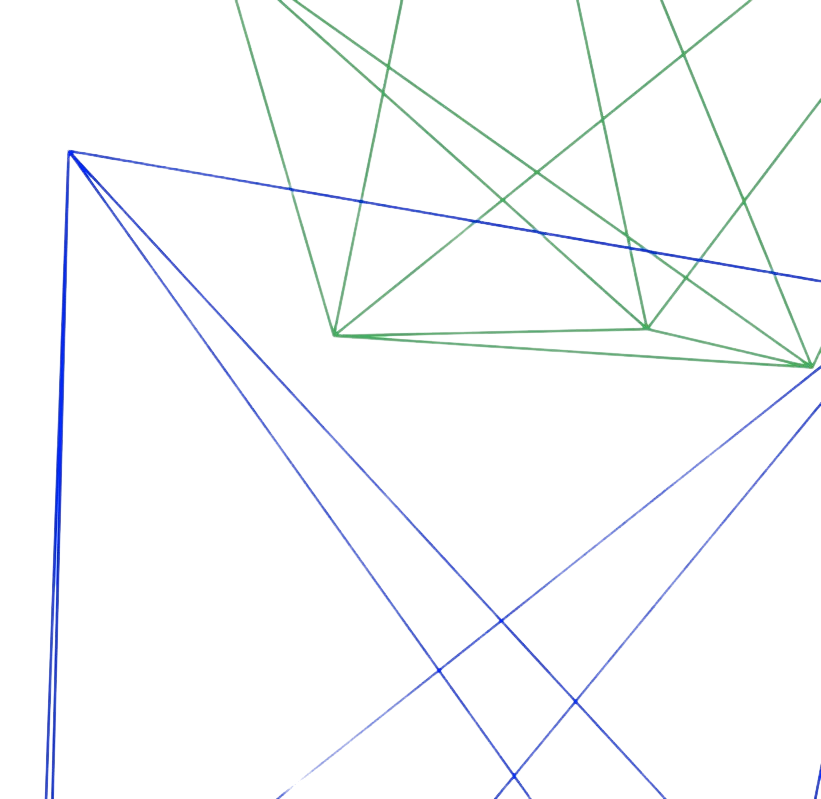
\includegraphics[width=0.5\paperwidth,height=\paperheight]{/root/.config/latex-utils/logos/invert1.png}};

        %\node[opacity=0.15, inner sep=0pt, anchor=south west] at (current page.south west){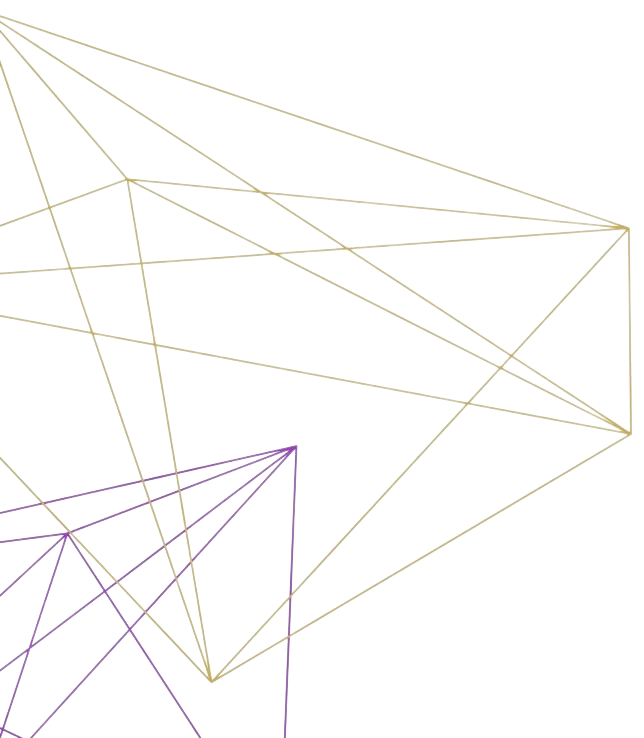
\includegraphics[width=0.5\paperwidth,height=0.5\paperheight]{/root/.config/latex-utils/logos/invert2.png}};

        \node[opacity=0.1,inner sep=0pt, anchor=north west] at (current page.north west){
\includegraphics[width=0.5\paperwidth,height=0.5\paperheight]{/root/.config/latex-utils/logos/invert3.png}};

        % Empressarios Logo
        \fill[fill=gray!30, opacity=0.75] (page cs: 1,0.545) -- (page cs: -1,0.545) -- (page cs: -1,0.768) -- (page cs: 1,0.768) -- (page cs: 1,0.545);
        \draw[line width=2.6pt] (page cs: 1,0.545) -- (page cs: -1,0.545);
        \draw[line width=2.6pt] (page cs: 1,0.619) -- (page cs: -1,0.619);
        \draw[line width=2.6pt] (page cs: 1,0.694) -- (page cs: -1,0.694);
        \draw[line width=2.6pt] (page cs: 1,0.768) -- (page cs: -1,0.768);
        \fill[thin, fill=red, opacity=1] (page cs: 0.96,0.561) -- (page cs: 0.649,0.561) -- (page cs: 0.684,0.603) -- (page cs: 0.925,0.603) -- (page cs: 0.96,0.561);
        \fill[thin, fill=red, opacity=1] (page cs: 0.605,0.561) -- (page cs: 0.339,0.561) -- (page cs: 0.374,0.603) -- (page cs: 0.64,0.603) -- (page cs: 0.605,0.561);
        \fill[thin, fill=red, opacity=1] (page cs: 0.4,0.635) -- (page cs: 0.435,0.678) -- (page cs: 0.7,0.678) -- (page cs: 0.665,0.635) -- (page cs: 0.4,0.635);
        \fill[thin, fill=red, opacity=1] (page cs: 0.461,0.709) -- (page cs: 0.496,0.752) -- (page cs: 0.761,0.752) -- (page cs: 0.726,0.709) -- (page cs: 0.461,0.709);
        \fill[thin, fill=red, opacity=1] (page cs: 0.71,0.635) -- (page cs: 0.745,0.678) -- (page cs: 0.865,0.678) -- (page cs: 0.9,0.635) -- (page cs: 0.71,0.635);
        \fill[thin, fill=red, opacity=1] (page cs: 0.77,0.709) -- (page cs: 0.805,0.752) -- (page cs: 0.84,0.709) -- (page cs: 0.77,0.709);

        \node at (page cs:-0.65,0.731) {\fontsize{21}{25.2}\bfseries\textit{EMPRESSARIOS}};
        \node at (page cs:-0.7,0.657) {\fontsize{21}{25.2}\bfseries\textit{AGRUPADOS}};
        \node at (page cs:-0.63,0.582) {\fontsize{21}{25.2}\bfseries\textit{INTERNACIONAL}};


        \node at (page cs:0,0.875) {\Large\bfseries\textsc{BUT GEII - CITISE}};
        \node at (page cs:0,0.925) {\LARGE\bfseries\textsc{Telecom Saint-Étienne}};

        \node at (page cs:0.5,-0.1) {\Large\textsc{Luis Cerrada Duque - Tuteur entreprise}};
        \node at (page cs:0.63,-0.15) {\Large\textsc{Viktor Fischer - Tuteur IUT}};







        %\node[opacity=0.15, inner sep=0pt, anchor=south west] at (current page.south west){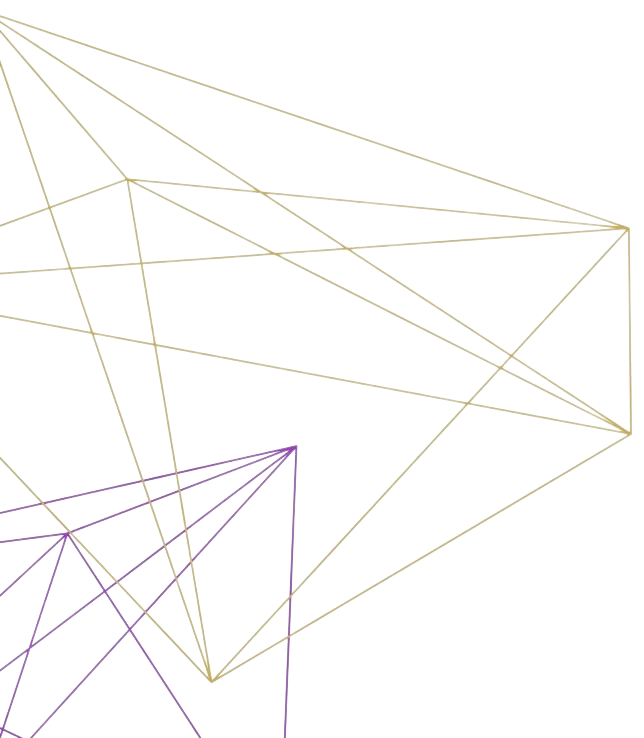
\includegraphics[width=0.5\paperwidth,height=0.5\paperheight]{/root/.config/latex-utils/logos/invert2.png}};

        \node at (page cs:0,0.4) {\fontsize{28}{28.8}\textbf{\ctoptitle}};
        \node at (page cs:0,0.325) {\fontsize{28}{28.8}\textbf{\ctitle}};
        \draw (page cs:0.5,0.275) -- (page cs:-0.5,0.275);
        \node at (page cs:0,0.245) {\Large\textsc{Stage de Technicien en Gênie Électrique et Informatique Industrielle}};
        \node at (page cs:0,0.17) {\Large\textsc{17.14.2023 - 23.06.2023}};
        \node at (page cs:0,0.210) {\Large\bfseries\textsc{Empresarios Agrupados Internacional}};
        \node at (page cs:0,0.135) {\LARGE\textsc{\cautor}};

        \node at (page cs:0,0.9) {
\includegraphics[height=1.5cm]{./1.png}\hspace{0.3cm}
\includegraphics[height=1.5cm]{./2.png}\hspace{13cm}
\includegraphics[height=1.5cm]{/root/.config/latex-utils/logos/UJM.png}};
        % Telecom Logo Big
    \end{tikzpicture}

    \begin{tikzpicture}[remember picture,overlay,every node/.style={anchor=south west}]
        \fill[thin, fill=ccolor1, opacity=1] (page cs: -1,-0.39) arc (124.5:-4.7:10cm) -- (page cs: -1,-1) -- (page cs: -1,-0.39);
        \fill[thin, fill=ccolor2, opacity=1] (page cs: -1,-0.14) arc (92.3:53.25:10cm) arc (85.9:124.5:10cm) -- (page cs: -1,-0.14);
        \fill[thin, fill=ccolor3, opacity=1] (page cs: -1,-0.005) arc (106:18.7:10cm) arc(49:85.9:10cm) arc (53.25:92.3:10cm) -- (page cs: -1,-0.005);
        \fill[thin, fill=ccolor4, opacity=1] (page cs: -0.06,-1) arc (-16.65:52.5:10cm) arc (85.9:49:10cm) arc (18.7:-34:10cm) -- (page cs: -0.06,-1);
        \fill[thin, fill=white, opacity=1] (page cs: -0.17,-1) -- (page cs: -0.17,-0.523) -- (page cs: -0.525,-0.374) -- (page cs: -1,-0.57) -- (page cs: -1,-1) -- (page cs: -0.925,-1) -- (page cs: -0.925,-0.833) -- (page cs: -0.515,-0.665) -- (page cs: -0.515,-1) -- (page cs: -0.17,-1);
    \end{tikzpicture}
\end{titlepage}

\newgeometry{left=2.5cm, width=16cm, bottom=2.5cm, top=2.5cm}
\thispagestyle{plain}
\textcolor{white}{Blank page}


\newpage
\thispagestyle{plain}
\begin{tikzpicture}[remember picture,overlay,every node/.style={anchor=south west}]
    \node at (page cs: 0,0.25) {\huge\bfseries\textsc{Création de Liste de Signaux et Logique}};
\end{tikzpicture}


\newgeometry{width=16cm, bottom=2cm, top=2cm}

\tikz[remember picture, overlay] \node[opacity=0.15,inner sep=0pt, anchor=north east] at (current page.north east){
\includegraphics[angle=-90,origin=c,width=0.5\paperheight,height=0.5\paperwidth]{/root/.config/latex-utils/logos/invert3.png}};
\tikz[remember picture,overlay] \node[opacity=0.15,inner sep=0pt, anchor=south east] at (current page.south east){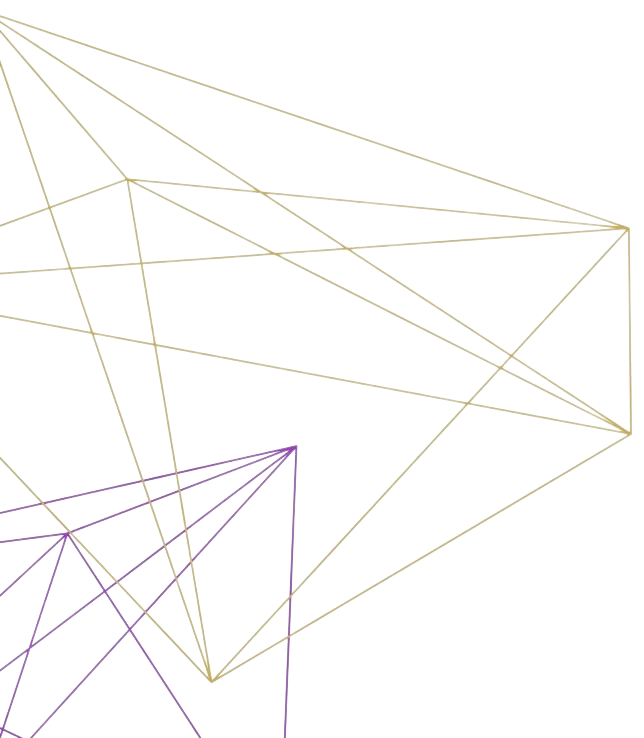
\includegraphics[angle=90,width=0.5\paperwidth,height=0.5\paperheight]{/root/.config/latex-utils/logos/invert2.png}};

\tableofcontents

\newgeometry{left=2.5cm, width=16cm, bottom=2.5cm, top=2.5cm}



